\section{Spectra analysis}
\label{sec:spectraanalysis}
For the can detector, the approximate sweet spot for Am and Fe were rough gain of $4$ and bias voltage of $1937$ V. The measurement times are listed in Tab.~\ref{tab:measurementstimes}. For the can detector, the sources were collimated.

In this section, the figures of the spectra taken with the aluminium detector assumbled by group 2 and with the can detector will be shown side-by-side with the can detector on the left and the aluminium detector on the right. The spectra from the aluminium detector were collected at a gain of $10$ and bias voltage of $1217$ V.

\begin{table}[htb]
  \centering
\begin{tabular}{lll}
\textbf{Detector}    & \textbf{Source} & \textbf{Live time {[}min.{]}} \\ \hline
\multirow{3}{*}{Can} & Fe-55           & 5                          \\
                     & Am-241          & 15                         \\
                     & Bkg             & 45                         \\ \hline
\multirow{3}{*}{Alu} & Fe-55           & 19                         \\
                     & Am-241          & 25                         \\
                     & Bkg             & 30                         \\ \hline
\end{tabular}
\caption{List of measurement times for the different sources and setups.}
\label{tab:measurementstimes}
\end{table}

\begin{figure*}[htb]
  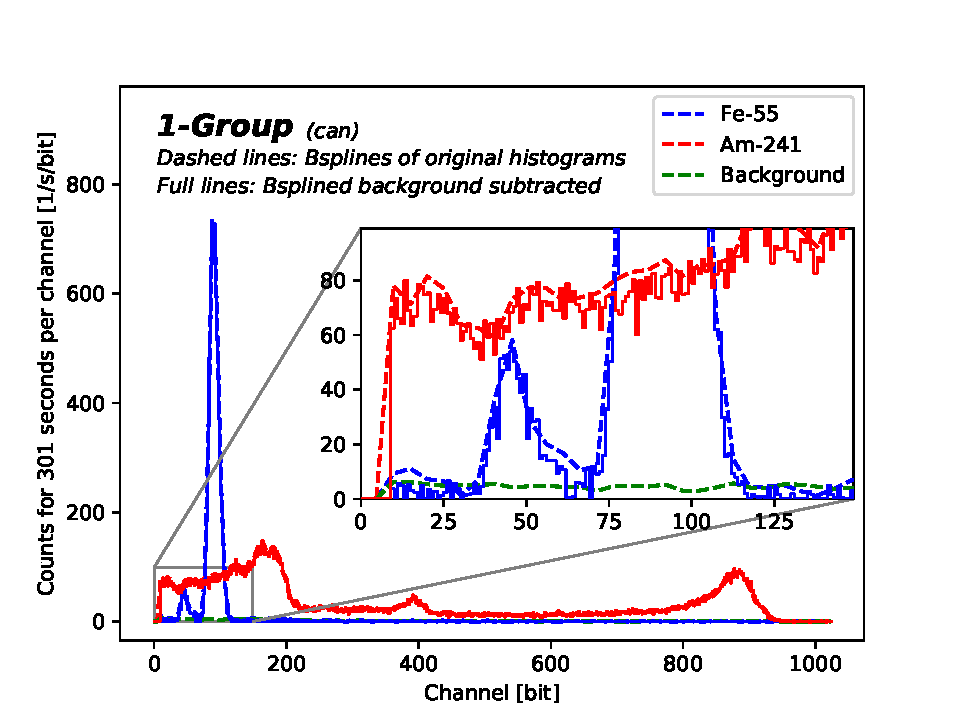
\includegraphics[width=0.49\textwidth,page=1]{graphics/bkgsubtraction.pdf}
  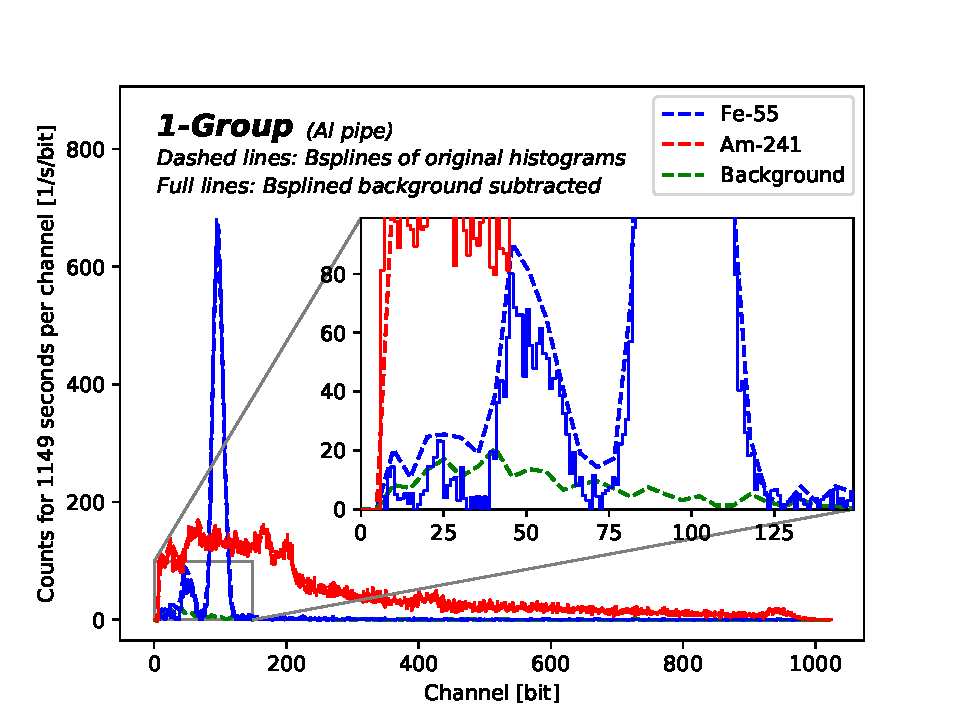
\includegraphics[width=0.49\textwidth,page=1]{graphics/alubkgsubtraction.pdf}
  %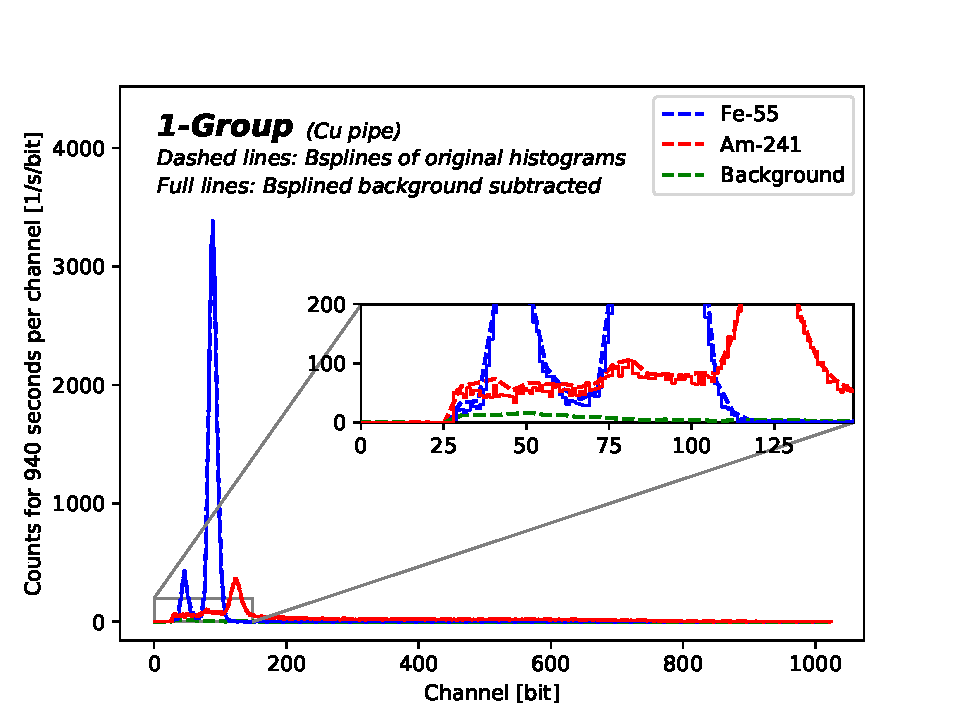
\includegraphics[width=0.32\textwidth,page=1]{graphics/cupbkgsubtraction.pdf}
  \caption{Spectra of Fe and Am as well as background for the can detector and the aluminium detector. Am and background have been normalised to the Fe spectra. The dashed lines are splines of the original histograms, and the full lines are the splined sources with splined background subtracted. The shown resolution of the splines is intentionally low.}
  \label{fig:spectra}
\end{figure*}

When the sources are measured, the data files are loaded into histograms which are then converted to cubic basis splines (B-splines) with smoothing of 0.02 for the sources and 0.002 for the background. These are shown as dashed lines in Fig.~\ref{fig:spectra}. The Am and background spectra are normalised to the Fe spectrum. The splined background is then subtracted from the splined sources and binned into 1024 bits and shown as the full lines in the figure. For the aluminium detector, the spline procedure does distort the escape peak somewhat. All subsequent figures will only be shown with the background subtracted.

Gaussian fits are then performed on the known Fe and Am peaks. All fits are performed using Chi-squared minimisation with square root of counts as uncertainties. Different fit functions are used and detailed in Tab.~\ref{tab:fitfuncchannelfits}. Fits are first performed with strict bounds which are then entirely lifted to show stability and for correctness of uncertainties. For the can detector, only bins with values larger than 20 are used for the escape peak and the Am peak as Chi-squared fits with square root uncertainties over-estimate the goodness-of-fit for bins with low counts. For the Fe double Gaussian, the fit spans further in order to reach convergence for the unbounded fit. For the aluminium detector, the escape peak is badly shaped, possibly due to the spline procedure. Therefore, the fit is performed from the right tail and above the peak until the shape deterioates. For the Fe double Gaussian, some of the left side is left out to help convergence of the unbounded fit. For both detectors, the left side of the Am peak is not well modeled by a single Gaussian peak, wherefore it is mostly left out from the fit.

For the escape peak fits, a regular Gaussian is used. For the Fe peak, the uncorrelated double Gaussian is used. For the Am peak, a regular Gaussian is used for the can detector. However, for the aluminium detector, a 1st order polynomial must be added to ensure convergence.

\begin{table*}[htb]
  \centering
\begin{tabular}{ll}
\textbf{Name}                 & \textbf{Expression} \\ \hline
Gaussian                      & $\frac{N}{\sqrt{2\pi}\sigma}\exp{\left(-\frac{\left(x-\mu\right)^2}{2\sigma^2}\right)}$                    \\
Uncorrelated double Gaussian  & $N\left[r\frac{1}{\sqrt{2\pi}\sigma}\exp{\left(-\frac{\left(x-\mu\right)^2}{2\sigma^2}\right)}+(1-r)\frac{1}{\sqrt{2\pi}\sigma}\exp{\left(-\frac{\left(x-\mu\right)^2}{2\sigma^2}\right)}\right]$                     \\
Gaussian plus 1st order poly. & $\frac{N}{\sqrt{2\pi}\sigma}\exp{\left(-\frac{\left(x-\mu\right)^2}{2\sigma^2}\right)} + b + ax$                   
\end{tabular}
\caption{Expressions for the used fit functions for the Gaussian fits. These are regular Gaussian functions with a normalisation factor. The uncorrelated double Gaussian expression is used for fits with overlapping signals, and has less correlated parameters than two regular Gaussians. The parameters are the usual Gaussian parameters as well as the normalisation factor, $N$, the ratio, $r$, and the polynomial factors, the y-intersection, $b$, and the slope, $a$.}
\label{tab:fitfuncchannelfits}
\end{table*}

\begin{figure*}[htbp]
  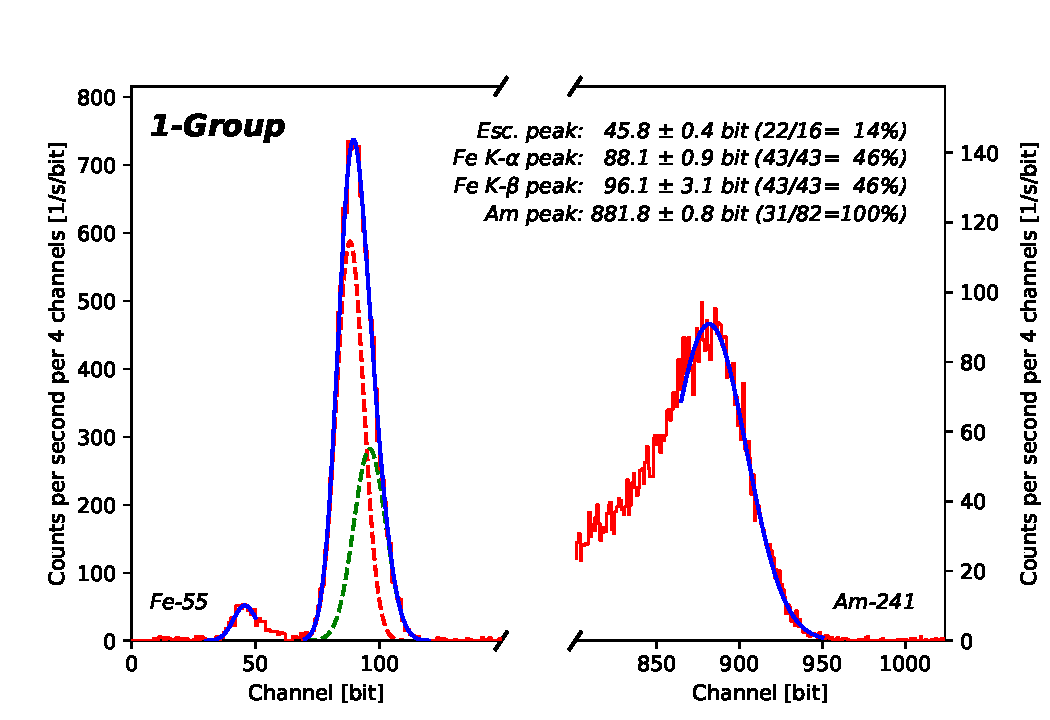
\includegraphics[width=0.49\textwidth,page=1]{graphics/channelfits.pdf}
  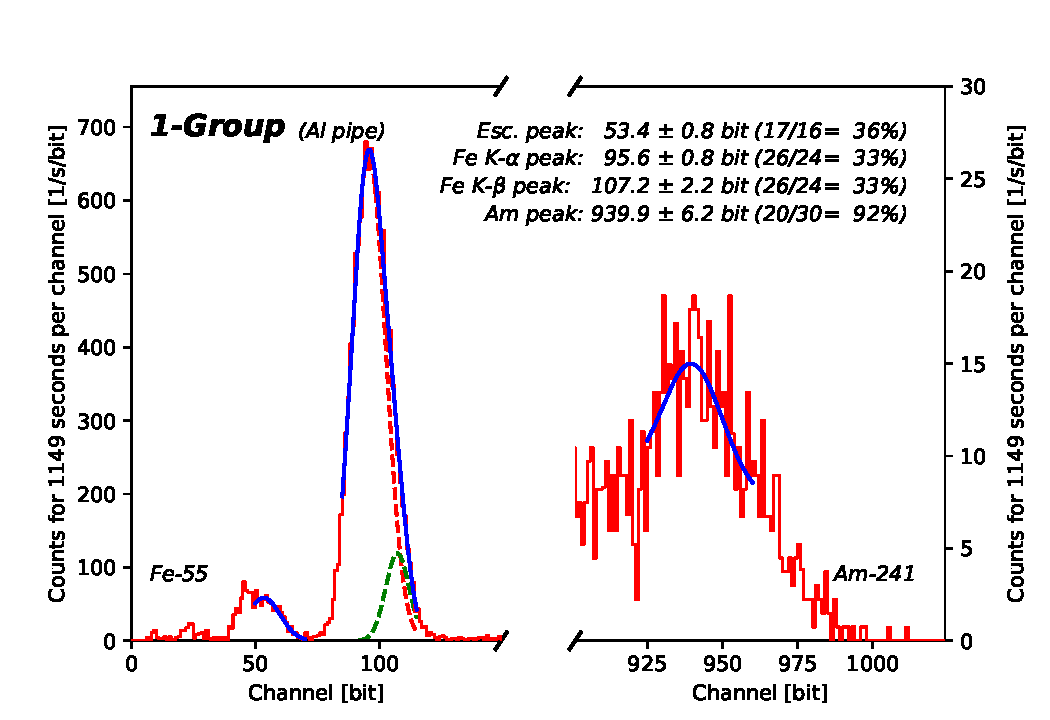
\includegraphics[width=0.49\textwidth,page=1]{graphics/aluchannelfits.pdf}
  \caption{Fits to the four known peaks, the escape peak, the double iron, and the americium. The single Gaussians of the double iron peak are shown as dashed lines. The resulting centroids of the fits are shown in the figure along with the Chi-squared value, number degrees of freedom, and the Chi-squared probability. Note the broken x-axis.}
  \label{fig:channelfits}
\end{figure*}

After extracting the centroids, the four peaks are plotted against their known energies and a 1st order polynomial fit is performed. The result is shown in Fig.~\ref{fig:energychannelcalib}. For the aluminium detector, the low Chi-squared value is due to the larger uncertainties coming from the poor Gaussian fits, and the y-intersection is not consistent with 0.

\begin{figure*}[htbp]
  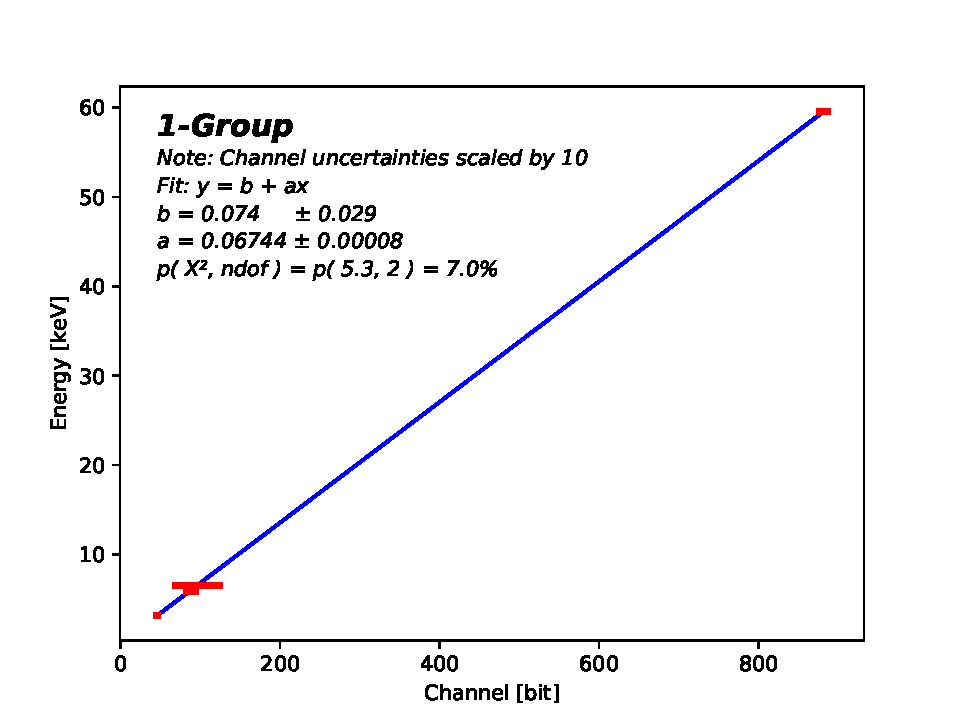
\includegraphics[width=0.49\textwidth,page=1]{graphics/energychannelcalib.pdf}
  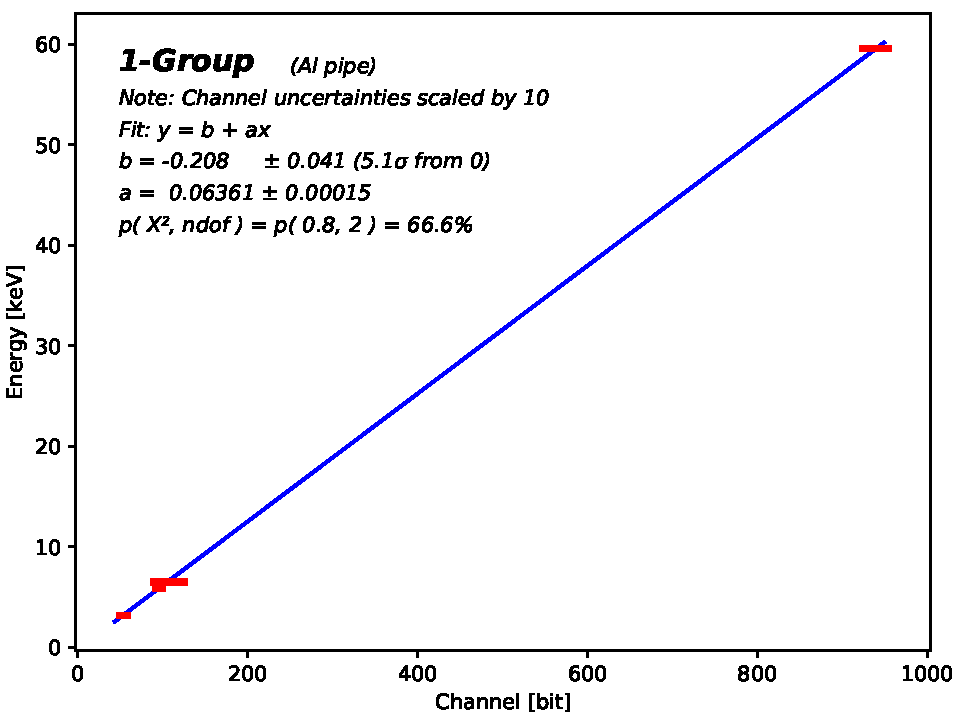
\includegraphics[width=0.49\textwidth,page=1]{graphics/aluenergychannelcalib.pdf}
  \caption{The centroids found in Fig.~\ref{fig:channelfits} are plotted against their known energies and fitted with a 1st order polynomial. The y-intersection is not fixed. For the can detector, the uncertainties on the data points are reasonable, while for the aluminium detector, the large uncertainties lead to a smaller Chi-squared value. For the aluminium detector, the y-intersection is also not consistent with 0. Note that the uncertainties are scaled by 10 to aid visualization.}
  \label{fig:energychannelcalib}
\end{figure*}

With the calibration for conversion of channel to energy, the additional peaks in the americium spectra will be fitted. The result is shown in Fig.~\ref{fig:peaksearch}. For the aluminium detector, due to the poor quality, only the biggest of the small peaks were fitted. For this peak, a Gaussian with a 1st order polynomial was used, and the same procedure as before was followed.

For the can detector, four peaks were fitted individually with only peak 1 left in a bound fit. All four fits were made with a Gaussian plus a 1st order polynomial. Afterwards, all 4 peaks were fit simultaneously with 4 Gaussians on a 1st order polynomial background. The starting values used were the Gaussian parameters from the previous fits with a $\pm 20\%$ bound. However, the widths of the smaller peaks, 2 and 3, were fixed in the simultaneous fit. The starting values for the polynomial were approximately set with very loose bounds.

In Fig.~\ref{fig:peaksearch}, the energy uncertainties of the peaks are shown split into its statistical, calibrational, and systematical components. Tab.~\ref{tab:peakschannelenergies} shows the fully combined uncertainties only.

\begin{figure*}[htbp]
  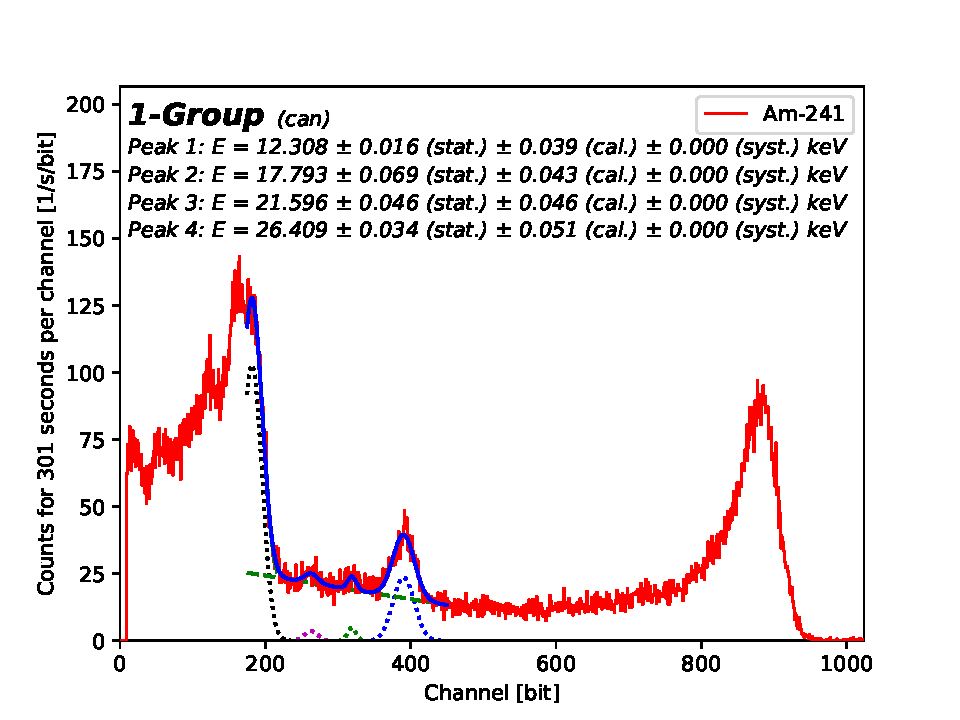
\includegraphics[width=0.49\textwidth,page=1]{graphics/peaksearch.pdf}
  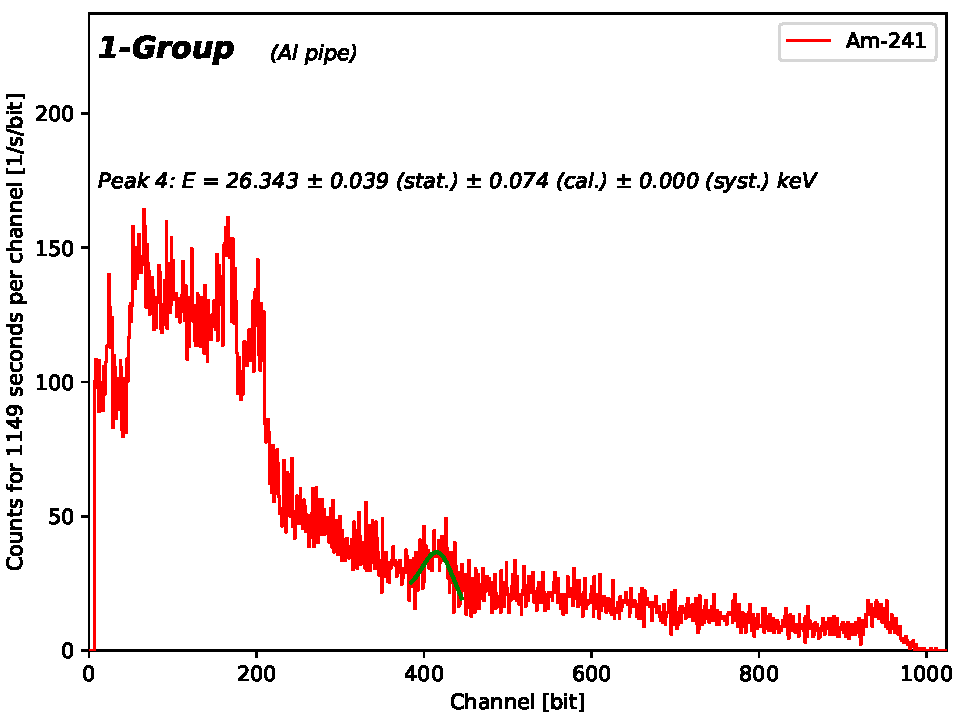
\includegraphics[width=0.49\textwidth,page=1]{graphics/alupeaksearch.pdf}
  \caption{Additional peaks in the americium spectrum are fitted. For the can detector, the individual components of the 4 Gaussians fit are shown in dashed lines. See the text for the fitting details.}
  \label{fig:peaksearch}
\end{figure*}

\begin{table*}[htbp]
  \centering
\begin{tabular}{lrrrr}
              & \multicolumn{2}{c}{\textbf{Can}} & \multicolumn{2}{c}{\textbf{Alu}} \\
\textbf{Peak} & \textbf{Centroid [bit]}      & \textbf{Energy [keV]}      & \textbf{Centroid [bit]}     & \textbf{Energy [keV]}     \\ \hline
Esc.          & $ 45.90 \pm 0.55$ & $ 3.19$          & $ 53.39 \pm 0.84$ & $ 3.19$          \\
Fe K-$\alpha$ & $ 88.11 \pm 0.91$ & $ 5.89$          & $ 95.64 \pm 0.80$ & $ 5.89$          \\
Fe K-$\beta$  & $ 96.06 \pm 3.13$ & $ 6.49$          & $107.21 \pm 2.22$ & $ 6.49$          \\
Am            & $881.11 \pm 1.06$ & $ 59.5$          & $939.23 \pm 1.92$ & $ 59.5$          \\
1             & $181.58 \pm 0.23$ & $12.31 \pm 0.79$ & -                 & -                \\
2             & $262.82 \pm 1.01$ & $17.79 \pm 1.14$ & -                 & -                \\
3             & $319.16 \pm 0.69$ & $21.60 \pm 1.38$ & -                 & -                \\
4             & $390.45 \pm 0.50$ & $26.41 \pm 1.69$ & $417.38 \pm 0.61$ & $26.34 \pm 0.08$ \\ \hline
\end{tabular}
\caption{List of measurement times for the different sources and setups.}
\label{tab:peakschannelenergies}
\end{table*}

The systematic uncertainty for the can detector is derived from the calibration of the preamplifier and the amplifier.
The MCA channel is a result of the original signal voltage amplified twice, leading to measurement of the form, $\textrm{channel} = f(G_\mathrm{pre} G_\mathrm{coarse} V)$.
Assuming linearity of the equipment, the relative uncertainty of the preamplifier and amplifier can be added in quadrature with the relative uncertainty of the centroids of the peaks.
The systematic uncertainty becomes rather large due to the coarse gain being derived from the scans that include the $\SI{10}{\percent}$ systematic uncertainty that accounts for the weakness of the resolution calculations.

Since the calibration of the preamplifier and the amplifier were only done for the can detector, no systematics have been derived for the aluminium detector.

The first, second and fourth peaks are consistent with a gamma-ray coming from Am-241 with energy of $\SI{26.34}{\kilo\electronvolt}$ \cite{amgammarays}.

\subsection{Copper pipe spectra}
Besides the data collected with the aluminium detector of group 2 and with the cider can detector, spectra were collected with a reference copper tube detector, see Sect.~\ref{sec:copper_construction}. The spectra from this detector were collected at a gain of $10$ and bias voltage of $1224$ V. The data analysis was conducted in the same manner as for the aluminium and cider can detectors, with the histograms being converted into cubic basic splines in order to subtract the background to the Fe and Am spectra. The Am and background spectra are normalised to the Fe spectrum. The spectra are shown is Fig.~\ref{fig:copperpipepeaks}, where the Fe spectrum resembles the one in Fig.~\ref{fig:spectra}, with the clear Fe peaks and the escape peaks in the same channels. On the other hand, the Am spectrum is quite different; the only clear peak is around channel $150$ and it could correspond to one of the unknown Am peaks in Tab.~\ref{tab:peakschannelenergies}. Smaller peaks are visible in the channel range $0-100$, and those could correspond to some of the noise visible in the same region in Fig.~\ref{fig:peaksearch} for both the aluminium and cider can detector. The Am peak of $59.5$ keV is not visible in this spectrum, a possible explanation to this could be that the gain was too high and the characteristic Am peak is then outside the probing window of MCA channels.

\begin{figure}[htbp]
  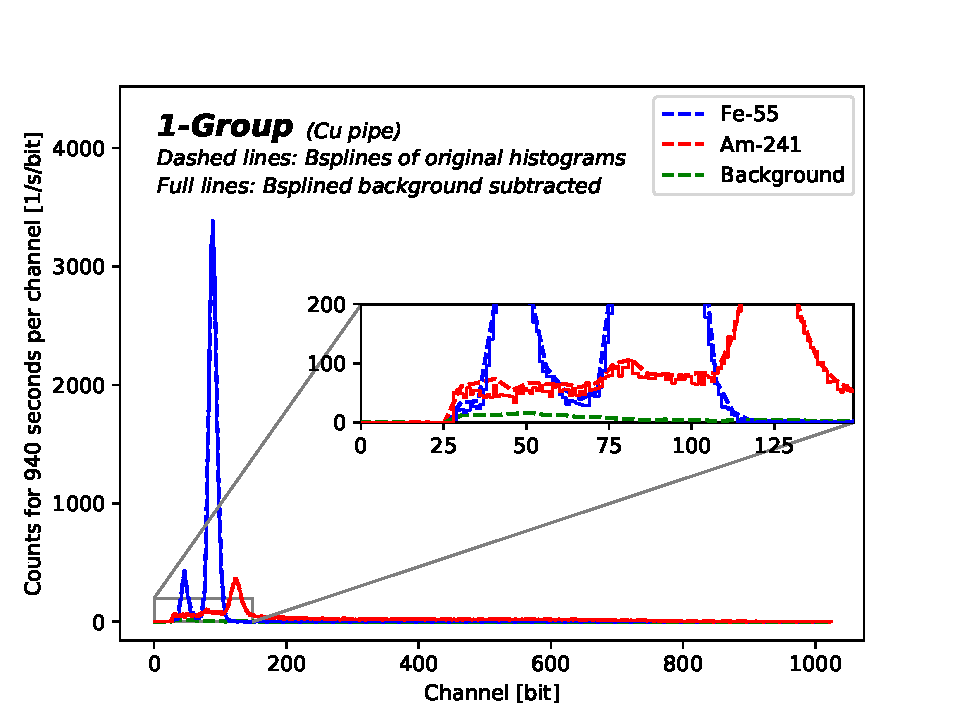
\includegraphics[width=0.5\textwidth]{graphics/cupbkgsubtraction.pdf}
  \caption{Spectra of Fe and Am as well as background for the copper pipe detector. Am and background have been normalised to the Fe spectra. The dashed lines are splines of the original histograms, and the full lines are the splined sources with splined background subtracted. The shown resolution of the splines is intentionally low.}
  \label{fig:copperpipepeaks}
\end{figure}
% There's a lot of figures here, and we better flush them out, so they don't mingle way further down the article
%\FloatBarrier
